\subsection{Noise Probebility Density Functions}

Her følger de mest almindelige PDF'er. Disse karakterisere de tilsyneladende tilfældige variabler som udgør støj i et billede.\\

I næste underafsnit beskrives Gaussian støj hurtigt, men udover denne er de andre:

\begin{itemize}
	\item Rayleigh
	\item Gamma
	\item Exponential
	\item Uniform
	\item Impulse
\end{itemize}

Deres kurver er alle vist i Figur~\ref{fig:noise-graphs}.

\subsubsection{Gaussian}

Er den mest normale slags støj, også vist på Figur~\ref{fig:noise-graphs}. Ligningen er vist på Figur~\ref{fig:gaussian-pdf}.

\begin{figure}[H]
	\centering
	
\includegraphics[width=0.7\linewidth]{figs/spm06/gaussian-pdf}
	\caption{Ligning for gaussian/normal støj.}
	\label{fig:gaussian-pdf}
\end{figure}

\begin{figure}[H]
	\centering
	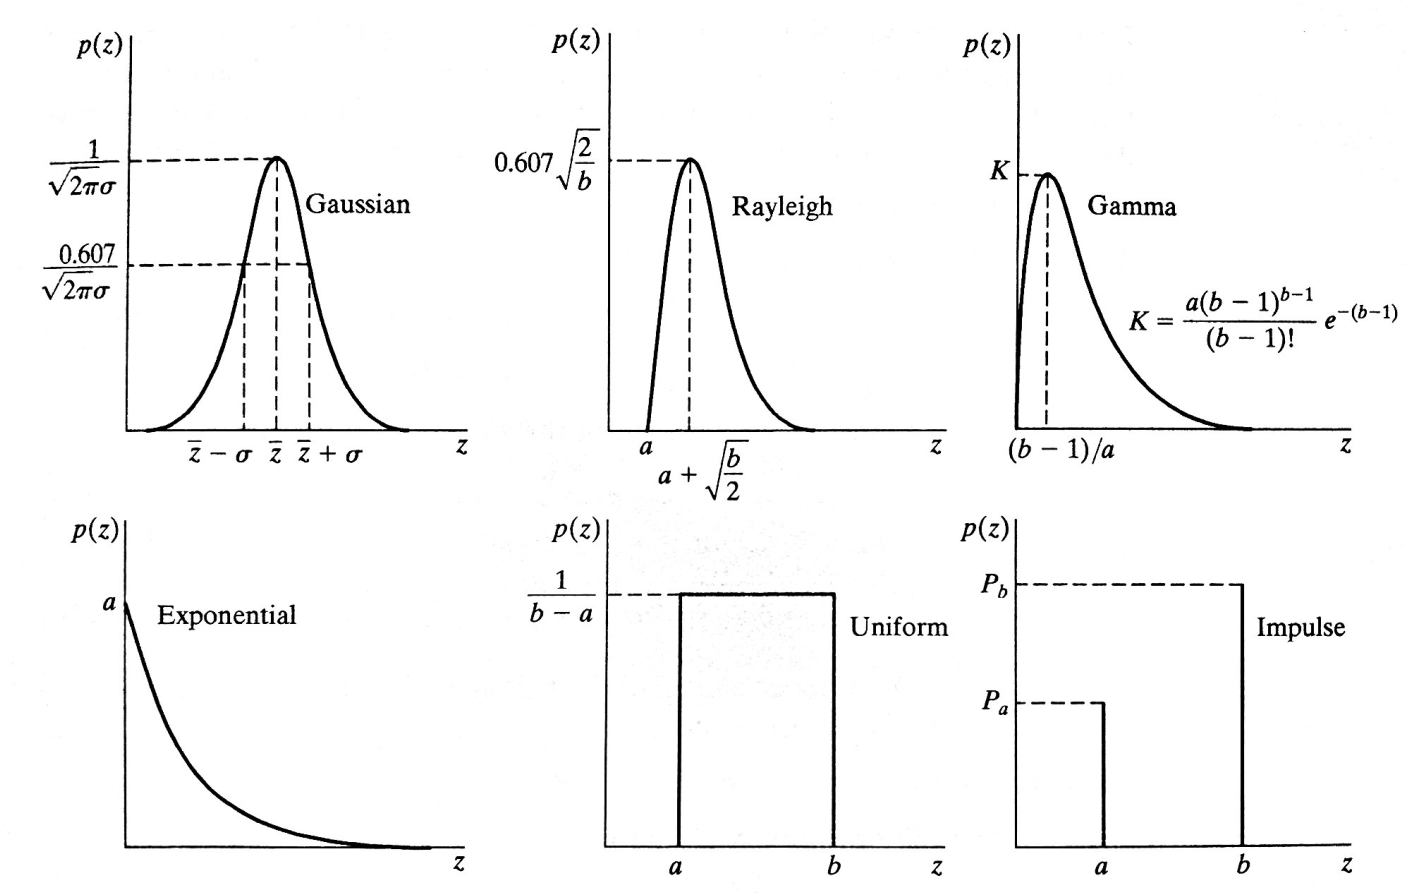
\includegraphics[width=\linewidth]{figs/spm06/noise-graphs}
	\caption{Forskellige typer af støj.}
	\label{fig:noise-graphs}
\end{figure}
